\documentclass[11pt,a4paper]{ivoa}
\input tthdefs

\usepackage{todonotes}
\usepackage{sidecap}

\lstloadlanguages{sh,SQL}
\lstset{flexiblecolumns=true,numberstyle=\small,showstringspaces=False,
  identifierstyle=\texttt,defaultdialect=[latex]tex,language=tex}

\definecolor{termcolor}{rgb}{0.6,0.1,0.1}
\newcommand{\vocterm}[1]{\emph{\color{termcolor}#1}}

\title{Adopting the UAT as an IVOA vocabulary}

% see ivoatexDoc for what group names to use here
\ivoagroup{Semantics}

\author[https://wiki.ivoa.net/twiki/bin/view/IVOA/MarkusDemleitner]{Demleitner, M.}
\author{Frey, K.}

\editor{Demleitner, M.}

\previousversion[http://ivoa.net/documents/uat-as-upstream/20201117/]{PEN-1.0-2021117}
       

\begin{document}
\begin{abstract}
The Unified Astronomy Thesaurus (UAT) provides a comprehensive, interlinked
set of concepts relevant for astronomy and astrophysics using SKOS.  It
is taken up in the Virtual Observatory at least for registry subject
keywords.  For various reasons, it is desirable to have the UAT
available subject to the constraints laid down in the IVOA Vocabularies in
the VO 2 specification.  This Note describes the rationale and the
details of the UAT adoption by the IVOA.
\end{abstract}



\section{Introduction}

Several components of the Virtual Observatory (VO) need to reference
concepts from astronomy and astrophysics, preferably in a uniform,
machine-readable way.  A rather prominent example is the \xmlel{subject}
element in the resource records described using VOResource
\citep{2018ivoa.spec.0625P}; other examples include \emph{Concept} in
VOEvent's \emph{Why} section \citep{2011ivoa.spec.0711S} or even SSAP's
target class \citep{2012ivoa.spec.0210T}.

Taking up, among other progenitors, earlier efforts within the
VO\footnote{See, in particular, section 4.5 for Vocabularies in the VO
1.13 \citep{2009ivoa.spec.1007G}; for the last version of the IVOA
thesaurus, see
\url{http://www.ivoa.net/rdf/Vocabularies/vocabularies-20091007/IVOAT/IVOAT.html}.},
the Unified Astronomy
Thesaurus\footnote{\url{https://astrothesaurus.org}} (UAT) gives a
comprehensive, interlinked set of such concepts that, contrary to the
IVOA thesaurus, is actively maintained.  
The American Astronomical Society already requires authors to
assign UAT keywords to articles published in their journals.

It therefore made sense for VOResource to adopt the UAT as the source
for its subject keywords.

In version 2, released in January 2017, the UAT 
moved to using language-neutral
concept URIs (as in \url{http://astrothesaurus.org/uat/1774} for the
concept labeled ``Virtual Observatories'' at the time of writing); while
this is certainly a positive step in a multilingual environment, in the
VO, which is essentially English-only, this is an unwelcome complication
against having human-readable concept designations.  In particular, such
resource identifiers would break searching with clear text words, for
instance in RegTAP \citep{2019ivoa.spec.1011D}.  Hence, introducing
custom identifiers and linking them to the UAT resource identifiers
turned out to be highly desirable.

These extra identifiers then open up the possibility to publish the UAT
with all guarantees of IVOA vocabularies, including the provision of
zero-tooling vocabularies in desise, the simple JSON-based vocabulary
format introduced in Vocabularies in the VO, version~2
\citep{2021ivoa.spec.0525D}.  This will, for instance, simplify
the implementation of registry validators or query expanders.

This document will first briefly discuss the current UAT maintenance,
then present the mechanisms of mapping the upstream UAT to the
IVOA-flavoured UAT, and conclude with a few illustrative examples for
how the IVOA-flavoured UAT might be used.

\subsection{Role within the VO Architecture}

\begin{figure}
\centering

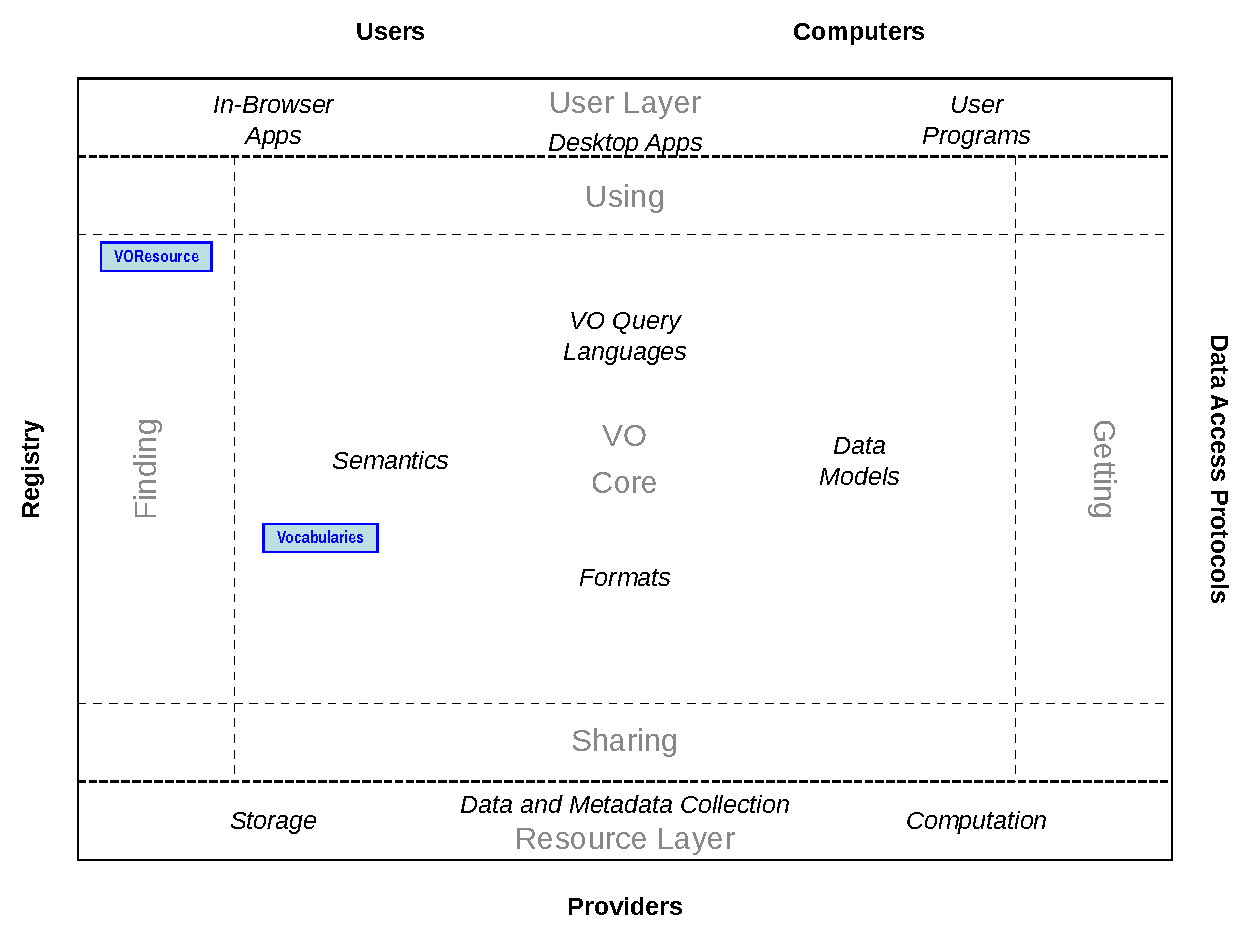
\includegraphics[width=0.9\textwidth]{role_diagram.pdf}
\caption{Architecture diagram for this Note}
\label{fig:archdiag}
\end{figure}

Fig.~\ref{fig:archdiag} shows the role this document plays within the
IVOA architecture \citep{2021ivoa.spec.1101D}.

This note is the normative basis for managing the IVOA artefacts for the
UAT as per Vocabularies in the VO 2 \citep{2021ivoa.spec.0525D}.  
It is, in particular,
required for realising the recommendation in VOResource 1.1
\citep{2018ivoa.spec.0625P} to use the UAT to assign subject keywords.

\section{Upstream UAT Curation}

The UAT is the result of a cooperation between major stakeholders in
astronomy, including the ADS, journal publishers, and the IVOA Semantics
group \citep{2014ASPC..485..461A}.  Since it is available under CC-BY-SA, 
no major legal barriers exist for re-dissemination by the IVOA.

A steering committee oversees the adoption of new terms as well as the
modification or deprecation of existing terms.  This steering committee
at this point consists of representatives of several libraries, the AAS,
the ADS, the CDS, and IOP publishing\footnote{See
\url{http://astrothesaurus.org/about/governance/} for a list of current
members.}.  Members of the steering committee have a two year term, with
the possibility of renewal.  A call for self-nominations to the
committee is distributed to various listservs around the time of the AAS
Annual meeting (January), and existing SC members vote on and select
from the pool of nominations in February.  Membership in the SC may be
drawn from astronomy societies, astronomy librarians, journal editors,
and other subject matter experts.

The UAT has a process for community
participation\footnote{\url{http://astrothesaurus.org/about/curation-process/}}
currently based on github.com's issue tracker, with a mandatory annual
review; conveniently from an IVOA perspective, the evaluation period for
such reviews runs from May to November and hence, roughly, from the
northen spring Interoperability Conference (that 
might thus be used to present major
changes) to the southern spring Interop (where the results of the review
process could be discussed).

In the past few years (2018-2020) the annual reviews updated between 100
and 600 concepts and added between 50 and 250.

It is our conviction that the processes employed by the UAT ensure
suffient community participation as well as continued evolution of the
thesaurus as the domain evolves.

\section{Mapping The Upstream UAT}

The adoption of the UAT as an IVOA-distributed vocabulary entails two
tasks:

\begin{enumerate}
\item The creation of human-readable concept identifiers.
\item The generation of the digital artefacts required by Vocabularies
in the VO 2.
\end{enumerate}

For task (1), we have developed a program uat2ivo maintained within
the UAT folder of the IVOA vocabulary source 
repository\footnote{\url{https://github.com/ivoa-std/Vocabularies/tree/master/uat}.}.

This program works on the RDF/XML representation that upstream UAT
keeps in its version control system.  At this point, it will follow the
UAT \emph{master} branch; an extra \emph{last-release} branch might be
considered if it turns out that updates beyond the regular UAT release
cycle become necessary.

The program maintains a stable mapping between UAT (numeric) concept
URIs and IVOA (human-readable) term URIs by parsing the RDF/XML
representation from the IVOA RDF repository (in \verb|ConceptMapping|'s
\verb|_fill_from_ivoa| method) and will only create new terms on the
IVOA side when new concept URIs are found in the upstream UAT.

The new terms are generated (in the \verb|label_to_term| function) by
replacing all runs of non-alphanumeric characters in the preferred label
with a single dash) and folding case to lowercase.  This yields UAT URIs
like

\begin{bigdescription}
\item[\url{http://www.ivoa.net/rdf/uat#achondrites}] from
\url{http://astrothesaurus.org/uat/15} (preferred label ``Achondrites'')
\item[\url{http://www.ivoa.net/rdf/uat#active-galactic-nuclei}]
from \url{http://astrothesaurus.org/uat/16} (preferred label ``Active
Galactic Nuclei'')
\item[\url{http://www.ivoa.net/rdf/uat#hubble-s-law}]
from \url{http://astrothesaurus.org/uat/763} (preferred label ``Hubble's
Law'')
\item[\url{http://www.ivoa.net/rdf/uat#kerr-newman-black-holes }]
from \url{http://astrothesaurus.org/uat/885} (preferred label
``Kerr-Newman black holes'')
\item[\url{http://www.ivoa.net/rdf/uat#l-galaxies}] from
\url{http://astrothesaurus.org/uat/895} (preferred label ``L galaxies'')
\end{bigdescription}

The program will add \vocterm{skos:exactMatch} elements to the new
SKOS concept it has created linking the new concept to the upstream UAT
concept.  Where new concepts are created, brief diagnostics are emitted
in order to raise the operator's attention in case of major malfunctions
in the mechanism that maintains the stable mapping.

In the event that a concept URI generated in this way collides with an
existing concept URI (which will happen if the preferred label folds
into the same string as a previous concept's preferred label at the time
of the generation of the mapping rule), the program will fail, and
manual resolution is necessary, either by changing the preferred label
or by adding a local override through uat2ivo's \verb|EXTRA_TRIPLES|.

These \verb|EXTRA_TRIPLES| -- a simple dictionary mapping UAT
identifiers to dictionaries of predicates and string values --
additionally contains some patches adding some triples for deprecated
UAT SKOS concepts; these include many preferred labels, as these are
necessary for creating a mapping, while the upstream UAT does not contain
them for many of the deprecated concepts.

As long as UAT releases happen about once per year, we plan to run the
updates manually; the chair of the Semantics WG will subscribe to the
release notifications and after a release manually run (adopted to
technology evolution as necessary), in a checkout of the vocabulary
sources\footnote{At the time of writing, 
\url{https://github.com/ivoa-std/Vocabularies}}:

\begin{lstlisting}[language=sh]
$ cd uat
$ python3 uat2ivo.py
$ cd ..
$ editor vocabs.conf  # update timestamp for UAT
$ git commit -am "Updating source for new UAT release"
$ python3 convert.py uat
\end{lstlisting}

This is then followed by the usual updating procedures.

Apart from oversight and the update to vocabs.conf (which can easily be
scripted as vocabs.conf is machine-readable),  no manual intervention is
necessary.  Thus, in case a more automated process is desired, this
update process could also run as part of continuous integration at the
UAT.

\section{UAT Applications and Use Cases}

\subsection{Using the UAT for VOResource Subject Keywords}

The main use of the IVOA-adopted UAT envisioned at this point is in
VOResource subjects.  Although the UAT has been adopted with VOResource
1.1 in 2018, initial uptake was very low, which is
understandable given that so far it was unclear whether to really include UAT
concept URIs, use preferred labels, or do something along the
lines of this proposal.

In 2020, the GAVO data center switched to using UAT key words as
proposed here; you can review the result of this procedure by running
a query like

\begin{minipage}{12cm}
\begin{lstlisting}[language=SQL]
SELECT 
  ivo_string_agg(res_title, '') AS title,
  ivo_string_agg(res_subject, ', ') AS subjects
FROM rr.resource
NATURAL JOIN rr.res_subject
WHERE ivoid LIKE 'ivo://org.gavo.dc%'
GROUP BY ivoid
\end{lstlisting}
\end{minipage}

\noindent on any RegTAP service (e.g., \url{http://reg.g-vo.org/tap}).

During the process, it became apparent that the current vocabulary could
be extended somewhat, in particular with a view to more
infrastructure-like services (e.g., validators, guides, or a generic
dataset-delivery service).  Efforts to remedy this lack are underway
using regular UAT procedures.



\subsection{Using the UAT for Discovery}

To investigate discovery modes enabled by the use of structured subject
keywords, a mapping of all existing subject keywords in the Registry to
UAT terms has been undertaken.  The result is available
online\footnote{\url{http://svn.ari.uni-heidelberg.de/svn/gavo/hdinputs/sembarebro/res/mapping.tsv}},
where items that were probably not UAT material were mapped to the
special value \emph{ivoa:None}, whereas terms that were not found in the
current UAT but might be considered as bases for UAT concepts later use
\emph{ivoa:TryAgain}.

This mapping was then used to create a custom RegTAP extension table,
\verb|rr.subject_uat|, which links mapped UAT concepts to IVOIDs of
Registered resources.  It is available on the TAP service at
\url{http://dc.g-vo.org/tap}.  This results in, at the time of writing,
about 420 UAT concepts for which VO resources are found.

\begin{SCfigure}
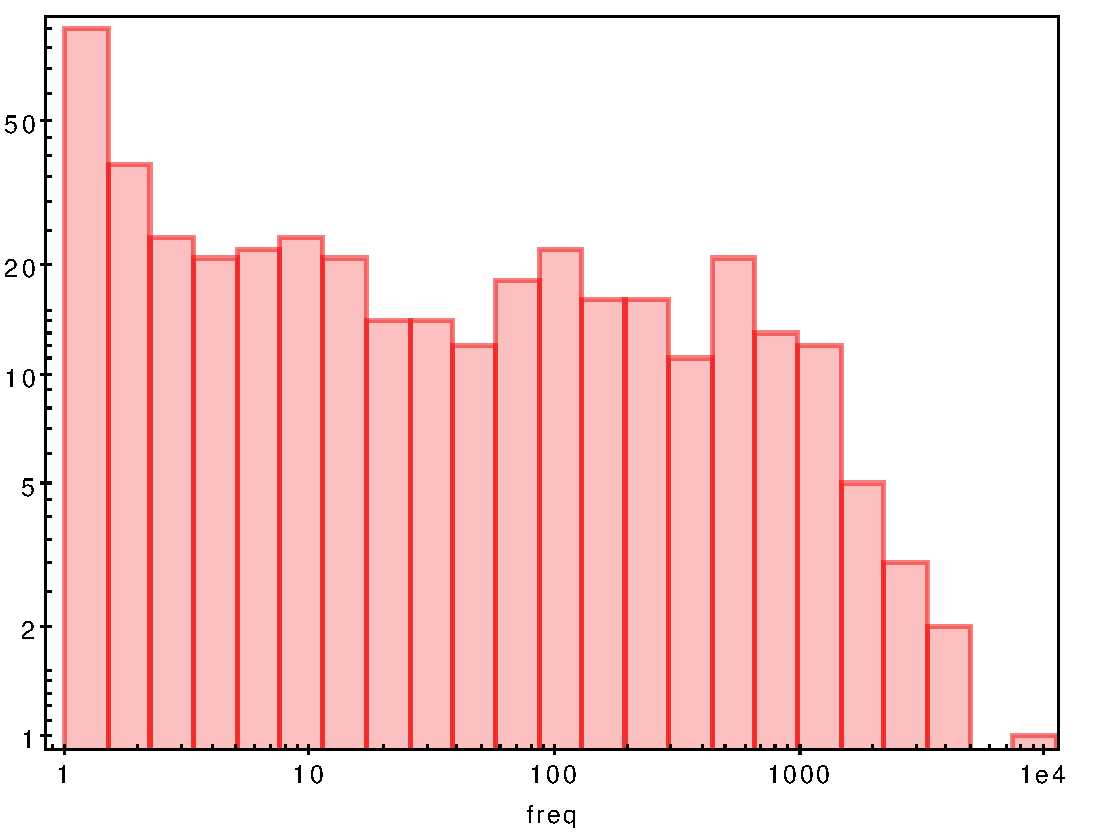
\includegraphics[width=7.5cm]{freqfreq.pdf}
\caption{The distribution of terms found with a given frequency (on the
x-axis) in a translation of subject keywords in the 2020 Virtual
Observatory.  Zipf's law predicts this should be a power law (i.e., a
straight line in this log-log plot)}
\label{fig:freqfreq}
\end{SCfigure}

Looking at the distribution of term frequencies, it turns out 
that it significantly flatter than 
the power law that Zipf's Law \citep{book:manning} would predict
here (cf.~Fig.~\ref{fig:freqfreq}).  We suspect this is an indication
that rarer concepts are under-represented, which in turn is probably due
to the translation from poorer schemes to the UAT.  In other words:
Using the richer set of UAT keywords can be expected to significantly
enrich the current metadata towards more precise concepts.

Based on the RegTAP extension, a semantics-based 
registry browser (or sembarebro for
short) was written as an experimental in-browser interface for resource
discovery in the VO\footnote{See
\url{http://dc.g-vo.org/sembarebro/q/ui/fixed}}.  The basic idea is
that, starting from some UAT concept, users can move around in the
UAT's concept graph and see if the concepts are represented in the VO
registry (see Fig.~\ref{fig:sembarebro}); the labels are 
rendered darker as more
resources match, and a click on the IVOA logos will take the user to a
list of the matching resources.

\begin{SCfigure}
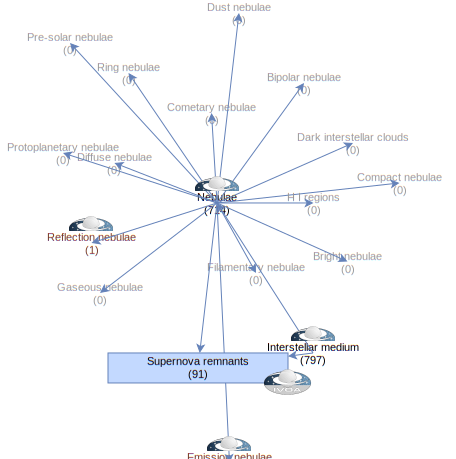
\includegraphics[width=8cm]{sembarebro.png}
\caption{A screenshot of a part of a sembarebro session; a part of the
UAT graph is shown, arrows going from wider to narrower terms.  VO
resources exist for the concepts with IVOA logos, and users can click on
labels to open up wider and narrower concepts.}
\label{fig:sembarebro}
\end{SCfigure}

The example shown in Fig.~\ref{fig:sembarebro} suggests another possible
use of UAT relationships in VO discovery. If a data provider did not evaluate
the full list of available UAT concepts and used ``nebulae'' to tag their
supernova remnants, and a user searches for nebula onlywould miss the
\vocterm{supernova-remnants}, along with \vocterm{interstellar-medium},
\vocterm{reflection-nebulae}, and \vocterm{emission-nebulae}. In this situation,
a user might be interested in resources tagged with nebulae and all resources
tagged with its UAT child concepts, as long as there aren't too many results.
And if there are too many results, then narrowing the query to 
\vocterm{supernova-remnants}
would cause the user to miss poorly tagged items.  As service
providers take up the more detailed UAT terms (and in perhaps less
contrived examples), isolating one's queries against different levels
of descriptions on the side of the resource record authors will become a
increasingly desirable.

The \verb|gavo_vocmatch| ADQL user defined function, which is being
prototyped in DaCHS \citep{2014A+C.....7...27D} since
version 2.2, mitigates this; it matches against a term and its narrower
neighbours (in the case of SKOS).  For instance, as of this writing,

\begin{minipage}{12cm}
\begin{lstlisting}[language=SQL]
SELECT DISTINCT ivoid 
FROM rr.resource
NATURAL JOIN rr.subject_uat
NATURAL JOIN rr.res_role
WHERE
  role_name LIKE 'Arias%'
  AND uat_concept='nebulae'
\end{lstlisting}
\end{minipage}

\noindent will miss data on the Cas A supernova remnant (although it indisputably
is a nebula)\footnote{Again, this example can be run on the TAP service
at \url{http://dc.g-vo.org/tap}.}.  Changing the last line to

\begin{lstlisting}[language=SQL]
    AND 1=gavo_vocmatch('uat', 'nebulae', uat_concept)
\end{lstlisting}

\noindent will return three resources, including 
the one on the supernova remnant,
as, we claim, users would expect.

\subsection{Other UAT Uses}

While we know of no concrete plans for the adoption of UAT concepts
within the IVOA except for
VOResource, it is likely that some other Virtual Observatory
standards might usefully employ the UAT.  

Considering the use cases mentioned in the introduction, the
SSAP/Obscore target class and VOEvent's \emph{Why}, one might argue that
in addition to clear and well-defined terms, which a simple adoption
of the UAT as-is would provide, having a strict tree of object
classes would be beneficial to data consumers.  The main advantage would
be that they could use a complete branch of narrower terms in query
expansion, which is not only very hard in a SKOS graph but also
inappropriate given that the relationsships in question are not
transitive.

Hence, it may be preferable to re-organise the object class-like
concepts from the UAT in such a strict tree (i.e., an RDF class
vocabulary in the nomenclature of Vocabularies in the VO 2) rather than
adopt the UAT directly.

\appendix
\section{Changes from Previous Versions}

\subsection{Changes from PEN-1.0-2021117}

Editorial changes only.

\bibliography{ivoatex/ivoabib,ivoatex/docrepo,local}


\end{document}
